% ============================================================================
% FreeGSNO model-architecture diagram  ---  standalone TikZ source for img/model.pdf
% main.tex (fig:integrated) includes the compiled img/model.pdf.
% To edit the figure: change the nodes/colors below, then regenerate with
%     pdflatex -output-directory=img img/model.tex      (run from the repo root)
%   or:  cd img && pdflatex model.tex
% ============================================================================
\documentclass[border=8pt]{standalone}
\usepackage{mathptmx}
\usepackage{amsmath,amssymb}
\usepackage{tikz}
\usetikzlibrary{arrows.meta,positioning,fit,backgrounds,calc}

% ---- palette ----
\definecolor{resInk}{RGB}{38,84,150}     % PI-DeepONet (residual) blue
\definecolor{resBg}{RGB}{234,241,251}
\definecolor{bndInk}{RGB}{176,86,0}      % PINTO (boundary) amber
\definecolor{bndBg}{RGB}{253,241,226}
\definecolor{outInk}{RGB}{31,122,77}     % output green
\definecolor{outBg}{RGB}{230,245,236}
\definecolor{ioInk}{RGB}{80,80,80}
\definecolor{ioBg}{RGB}{244,244,242}

\begin{document}
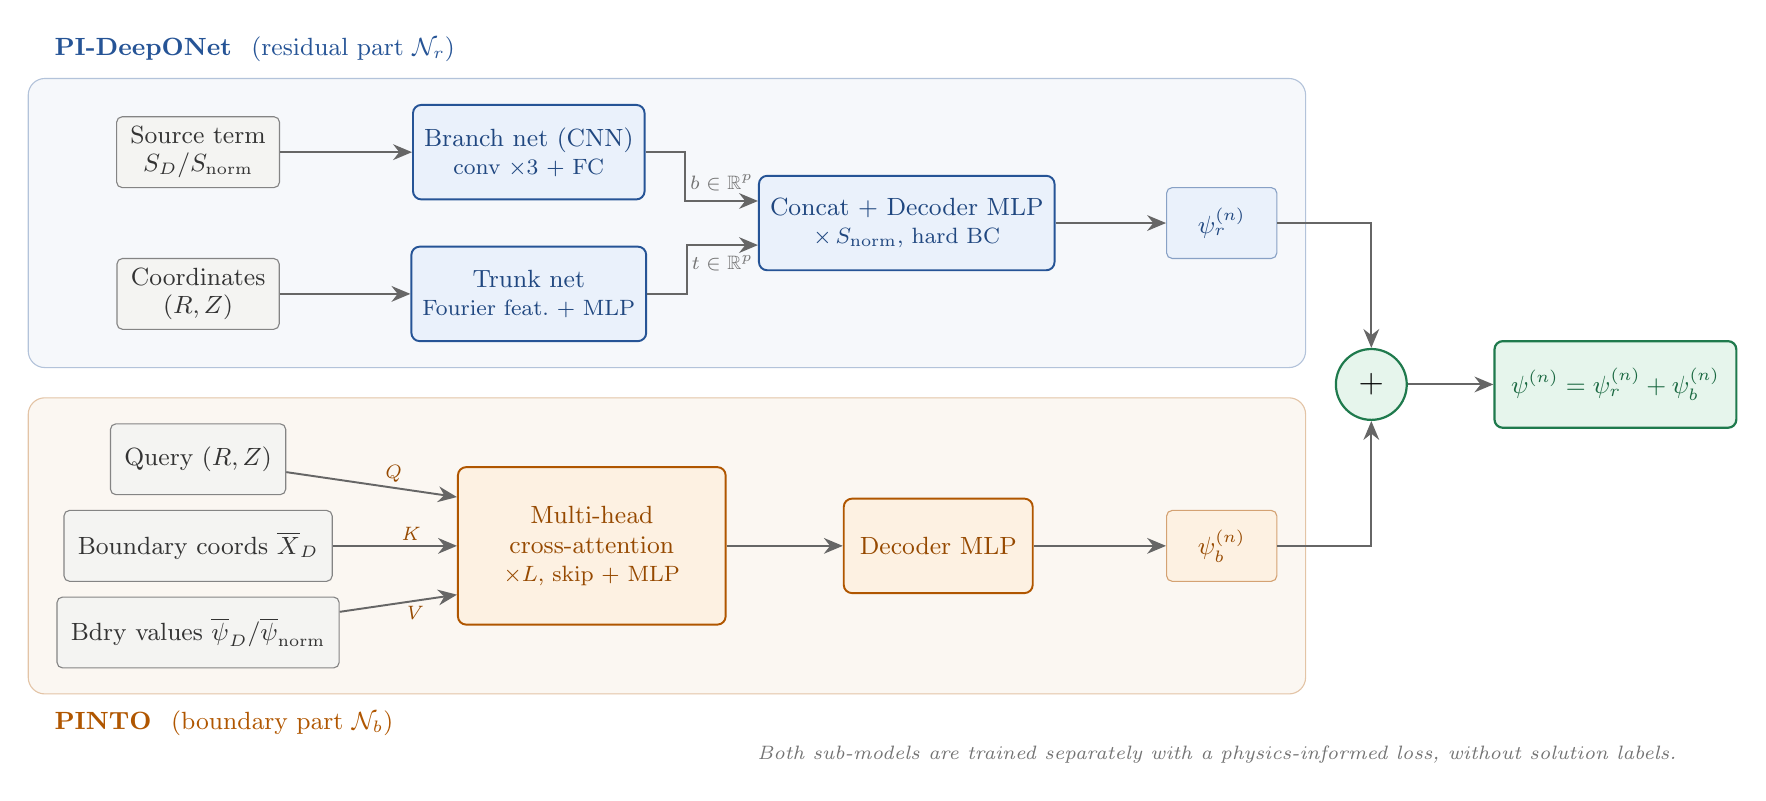
\begin{tikzpicture}[
  font=\small,
  io/.style   ={draw=ioInk!70, fill=ioBg, rounded corners=2pt, align=center,
                minimum height=9mm, inner xsep=5pt, inner ysep=3pt, text=black!80},
  bnet/.style ={draw=resInk, line width=.7pt, fill=resBg, rounded corners=3pt, align=center,
                minimum height=12mm, minimum width=26mm, inner sep=4pt, text=resInk!85!black},
  onet/.style ={draw=bndInk, line width=.7pt, fill=bndBg, rounded corners=3pt, align=center,
                minimum height=12mm, minimum width=26mm, inner sep=4pt, text=bndInk!85!black},
  merge/.style={draw=outInk, line width=.8pt, fill=outBg, circle, minimum size=9mm, inner sep=0pt},
  outbox/.style  ={draw=outInk, line width=.8pt, fill=outBg, rounded corners=3pt, align=center,
                minimum height=11mm, inner sep=6pt, text=outInk!85!black},
  flow/.style ={-{Stealth[length=2.4mm,width=2mm]}, line width=.7pt, draw=black!60},
  qkv/.style  ={font=\scriptsize\itshape, text=bndInk!85!black, inner sep=1.5pt},
  dim/.style  ={font=\scriptsize\itshape, text=black!55},
]

% ============ TOP LANE : PI-DeepONet (residual) ============
\node[io] (src)   at (0,6.5) {Source term\\[-1pt]$S_D/S_{\mathrm{norm}}$};
\node[io] (crd)   at (0,4.7) {Coordinates\\[-1pt]$(R,Z)$};

\node[bnet] (branch) at (4.2,6.5) {Branch net (CNN)\\[-1pt]\footnotesize conv $\times3$ + FC};
\node[bnet] (trunk)  at (4.2,4.7) {Trunk net\\[-1pt]\footnotesize Fourier feat.\ + MLP};

\node[bnet, minimum width=30mm] (dec) at (9.0,5.6)
  {Concat + Decoder MLP\\[-1pt]\footnotesize $\times\,S_{\mathrm{norm}}$,\ hard BC};

\node[io, draw=resInk!55, fill=resBg, text=resInk!85!black, minimum width=14mm]
  (psir) at (13.0,5.6) {$\psi_r^{(n)}$};

\draw[flow] (src)  -- (branch);
\draw[flow] (crd)  -- (trunk);
\draw[flow] (branch.east) -- ++(0.5,0) |- ($(dec.west)+(0,0.28)$)
   node[dim,pos=.75,above]{$b\in\mathbb{R}^{p}$};
\draw[flow] (trunk.east)  -- ++(0.5,0) |- ($(dec.west)+(0,-0.28)$)
   node[dim,pos=.75,below]{$t\in\mathbb{R}^{p}$};
\draw[flow] (dec) -- (psir);

% ============ BOTTOM LANE : PINTO (boundary) ============
\node[io] (qry) at (0,2.6) {Query $(R,Z)$};
\node[io] (key) at (0,1.5) {Boundary coords $\overline{X}_D$};
\node[io] (val) at (0,0.4) {Bdry values $\overline{\psi}_D/\overline{\psi}_{\mathrm{norm}}$};

\node[onet, minimum width=34mm, minimum height=20mm] (attn) at (5.0,1.5)
  {Multi-head\\ cross-attention\\[-1pt]\footnotesize $\times L$,\ skip + MLP};

\node[onet, minimum width=24mm] (decb) at (9.4,1.5)
  {Decoder MLP};

\node[io, draw=bndInk!55, fill=bndBg, text=bndInk!85!black, minimum width=14mm]
  (psib) at (13.0,1.5) {$\psi_b^{(n)}$};

\draw[flow] (qry) -- ($(attn.west)+(0,0.62)$) node[qkv,pos=.62,above]{Q};
\draw[flow] (key) -- ($(attn.west)+(0,0.0)$)  node[qkv,pos=.62,above]{K};
\draw[flow] (val) -- ($(attn.west)+(0,-0.62)$) node[qkv,pos=.62,below]{V};
\draw[flow] (attn) -- (decb);
\draw[flow] (decb) -- (psib);

% ============ MERGE ============
\node[merge] (sum) at (14.9,3.55) {\large$+$};
\node[outbox, minimum width=24mm] (out) at (18.0,3.55)
  {$\psi^{(n)}=\psi_r^{(n)}+\psi_b^{(n)}$};

\draw[flow] (psir.east) -| (sum);
\draw[flow] (psib.east) -| (sum);
\draw[flow] (sum) -- (out);

% ============ GROUP BACKGROUNDS (equal width, full coverage) ============
\begin{scope}[on background layer]
  % common horizontal extent over BOTH lanes
  \node[fit=(src)(crd)(branch)(trunk)(dec)(psir)(qry)(key)(val)(attn)(decb)(psib),
        inner xsep=10pt, inner ysep=0pt] (gall) {};
  % per-lane vertical extent (top box now includes crd & trunk)
  \node[fit=(src)(crd)(branch)(trunk)(dec)(psir), inner sep=9pt] (gtop) {};
  \node[fit=(qry)(key)(val)(attn)(decb)(psib),     inner sep=9pt] (gbot) {};
  \coordinate (topNW) at (gall.west |- gtop.north);
  \coordinate (topSE) at (gall.east |- gtop.south);
  \coordinate (botNW) at (gall.west |- gbot.north);
  \coordinate (botSE) at (gall.east |- gbot.south);
  \draw[draw=resInk!35, fill=resInk!4, rounded corners=6pt] (topNW) rectangle (topSE);
  \draw[draw=bndInk!35, fill=bndInk!5, rounded corners=6pt] (botNW) rectangle (botSE);
\end{scope}
\node[anchor=south west, font=\small\bfseries, text=resInk]
  at ([xshift=6pt,yshift=2.5pt]topNW) {PI-DeepONet\ \ \small\mdseries(residual part $\mathcal{N}_r$)};
\node[anchor=north west, font=\small\bfseries, text=bndInk]
  at ([xshift=6pt,yshift=-2.5pt]botSE-|topNW) {PINTO\ \ \small\mdseries(boundary part $\mathcal{N}_b$)};

% caption note
\node[anchor=east, font=\scriptsize\itshape, text=black!55, align=right] at (18.9,-1.15)
  {Both sub-models are trained separately with a physics-informed loss, without solution labels.};

\end{tikzpicture}
\end{document}
